% ----------------------------------------------------------
\chapter{Introdução}
\label{cap_intr}
% ----------------------------------------------------------
\section{Queimadas e Amazônia}
O Brasil é o país com a maior presença da floresta Amazônica na América, 60\% do total da floresta está dentro do território brasileiro, o que equivale a aproximadamente 5 milhões de quilômetros quadrados ou 59\% do território nacional \cite{tamanhoIBGE}. Por consequência disto, possuímos uma enorme responsabilidade com ela, existente em diversas formas, como na defesa do território nacional ou na proteção de um enorme patrimônio da humanidade. 

Tal patrimônio vem requerendo cada vez mais atenção nos últimos tempos, de acordo com dados gerados pelo PRODES \cite{novatecnica}, entre agosto de 2021 e julho de 2022 a taxa de desmatamento da Amazônia Legal foi cerca de 11594$km^{2}$. Como podemos ver na figura \ref{fig:prodesgraph}, tal taxa vem acompanhando uma alta nos últimos 10 anos do desmatamento no bioma. O INPE \cite{INPE} estima que, desde 1988, 17\% do bioma já tenha sido desmatado. Tais dados reforçam a necessidade de métodos de monitoramento e controle que reduzam as perdas do meio ambiente.

\begin{figure}[htb]
	\centering
	\begin{minipage}{0.9\linewidth}
		\centering
		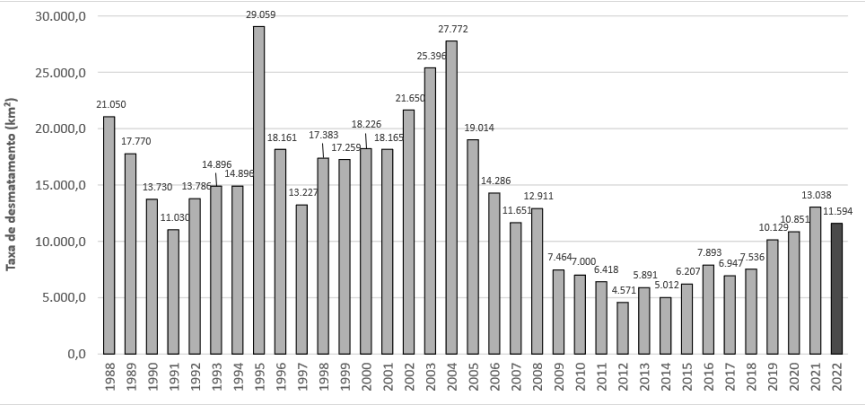
\includegraphics[width=\linewidth]{tg1/figuras/prodes.png}
		\caption{Taxas consolidadas anuais de desmatamento do PRODES \cite{novatecnica}}
            \label{fig:prodesgraph}
	\end{minipage}
\end{figure}

Uma importante área de atuação na preservação da floresta se trata do combate à incêndios. Todos os anos, milhares de quilômetros da floresta amazônicas são queimados por incêndios florestais, causando impactos ecológicos e econômicos, redução da biomassa florestal, mudanças na composição de espécies de árvores e esgotamento do solo \cite{penha}. 

Os incêndios podem ocorrer naturalmente ou podem estar atrelados a atividades humanas. No entanto, queimadas resultantes da ação humana constituem quase que a totalidade dos incêndios registrados nos territórios no Brasil, ocupando o 5º lugar entre os países mais poluidores \cite{bdqueimadas}.

Já as queimadas naturais, por sua vez, costumam ter sua ignição dada por raios, tornando-as mais comuns em períodos de secas prolongadas quando as queimadas costumam atingir seu pico. São mais frequentes no bioma Cerrado que é naturalmente mais seco e adaptado a queimadas naturais recorrentes, normalmente no início e fim das estações chuvosas. Em contraste, o bioma Amazônia é extremamente úmido e apresenta baixos índices de queimadas naturais.

Conforme pesquisas recentes \cite{amazonia_carbono}, a queima e o desflorestamento excessivo na floresta Amazônica estão afetando a capacidade de absorção de CO2 da atmosfera, ao mesmo tempo que estas atividades emitem grandes quantidades de carbono por meio da queima de madeira. Além disso, estas ações apresentam um impacto climático na região, tornando a estação seca mais seca, quente e longa, agredindo ainda mais o bioma.

\section{Objetivos}

Os incêndios florestais de origem antropológica são predominantemente e principalmente ligados ao desmatamento e a agricultura de manutenção \cite{severidade}. Nem todo fogo iniciado por atividade humana resultará em tragédia, mas a frouxidão das leis de proteção ambiental estimula pessoas mal intencionadas a queimar grandes áreas públicas para grilagem \cite{jornal_ambiental}, então ser capaz de controlar queimadas é importante tanto para proteger os bens naturais quanto para garantir a aplicação da legislação.

Dessa forma, este projeto visa criar uma ferramenta de \textbf{tipificação automática de incêndios} no território amazônico para auxiliar no combate ao fogo na região. De acordo com o \textit{EU Horizon 2020 Work Programme} \cite{horizon}, o ciclo de gestão do fogo pode ser amplamente segmentado em três etapas: (1) prevenção e preparação (pré-fogo); (2) detecção e resposta (gestão de incêndios florestais ativos); (3) atividades de restauração e adaptação (pós-incêndio). Este trabalho estará focado em desenvolver uma ferramenta que sirva de auxílio para a segunda etapa, na resposta dos órgãos de defesa para com incêndios ativos.

Este trabalho visou o desenvolvimento de um \textbf{algoritmo} projetado para ser incluído ao Painel do Fogo, uma plataforma Web que disponibiliza informações sobre incêndios e queimadas no Brasil, desenvolvido pelo Centro Gestor e Operacional do Sistema de Proteção da Amazônia \cite{painel-fogo}. No entanto, diferente de outras plataformas de monitoramento, o Painel do Fogo trabalha ao lado de batalhões e brigadas no combate ao fogo. Através desta plataforma se é possível obter o "perímetro" e o “status” mais recente sobre uma queimada ou incêndio de modo que um evento esteja associado a uma ocorrência ou acionamentos de equipes.

O modelo finalizado é capaz de \textbf{classificar queimadas} dentro das quatro classificações utilizadas pelo Censipam para tipificar incêndios florestais na Amazônia \cite{andela}: 

%O sistema foi treinado utilizando o extenso banco de dados de queimadas no território Amazônico oferecido pelo Amazon Dashboard do GFED \cite{gfed}. Estes dados são tratados e alimentados a um algoritmo de aprendizado de máquina para o treinamento. O modelo finalizado é capaz de classificar queimadas dentro das quatro classificações utilizadas pelo GFED para tipificar incêndios florestais \cite{andela}: 

\begin{itemize}
    \item  \textbf{Savana e pastagem}: vegetação de porte baixo, com pouca presença de biomassa, longa duração dias-semanas;
    \item \textbf{Pequenas clareiras}: pequenos incêndios em sistemas florestais (cobertura de árvores > 50$\%$ e igual ou inferior a 5 detecções de incêndios), curta duração, área menor que 100 ha;
    \item \textbf{Sub-bosque}: vegetação de porte arbustivo alto, Apresenta altas taxas de biomassa. Ocorre muito em borda de áreas desmatadas com floresta. Área variável, longa duração, poucos focos de calor por detecção, mesma região geográfica do desmatamento;
    \item \textbf{Desmatamento}: os incêndios de desmatamento normalmente têm alto poder radiativo inicial do fogo, pois os detritos lenhosos empilhados levam a uma maior liberação de energia e longa persistência do fogo, uma vez que essas pilhas podem arder por dias. Maior poder radiativo no início, maior duração, área variável.

\end{itemize} 

%Nosso objetivo é gerar nossa própria abordagem de tipificação, embora identificando os mesmos tipos de fogo e usando alguma instância de inteligência artificial, no que couber. No atual estado da arte, o GFED é o único dado a nível mundial com distribuição gratuita na internet que faz referência
%sobre tipos de fogo, mas não disponibiliza queimadas classificadas em tempo real. A diferença na data dos últimos dados disponibilizados para a data real é de cerca de um mês, propomos então um método que possa ser utilizado em tempo real para permitir rápida resposta dos órgãos de proteção ambiental.

A classificação de incêndios florestais desempenha um papel crucial na gestão ambiental, pois fornece informações essenciais para o desenvolvimento de estratégias de prevenção e combate ao fogo. Ao tipificar os incêndios dentro dessas categorias, as autoridades podem avaliar a ameaça que representam para a biodiversidade, comunidades humanas e ecossistemas. Essa análise permite a alocação eficiente de recursos, o planejamento de evacuações quando necessário e a mobilização de equipes de combate a incêndios. Além disso, a classificação de incêndios fornece dados valiosos para estudos e pesquisas que visam entender as causas subjacentes dos incêndios florestais e desenvolver medidas preventivas mais eficazes para proteger as florestas e o meio ambiente.

O Painel do Fogo já possui atualmente capacidade de tipificar seu banco de dados com as quatro classificações de queimada, porém o tempo e pessoal necessário para realizar tão avaliação não permite que estas informações possam ser incluídas na plataforma em tempo real junto com o atual produto da plataforma que é a visualização diária de novos eventos de fogo. O projeto é responsável por realizar tal trabalho de forma ligeira e com um bom nível de acurácia.

Para este fim, a plataforma fará uso de sistemas de \textbf{aprendizado de máquinas} para tipificar queimadas em curso, integrando estas informações à plataforma Web. Através dela, as informações são disponibilizadas para todos que tenham interesse e alertas serão emitidos para os agentes competentes conforme a necessidade.

O uso de inteligência artificial para cuidados durante o ciclo do fogo não são uma novidade, em \cite{invention} foi feita uma revisão de diversos artigos publicados entre 2019 e 2022 que tratavam do uso de métodos de aprendizado de máquina no controle de queimadas florestais. O que se pode concluir da revisão é que existe um potencial para a adoção de métodos de aprendizado de máquina para previsão e classificação e para melhorar o suporte às decisões gerais no monitoramento de danos ambientais relacionados ao fogo.

Em conjunto com um algoritmo de monitoramento, é necessário que acoplado a ele exista um método de fornecimento de dados. A maneira mais comum atualmente de se obter informações do estado mais recente do vasto território da floresta amazônica é por meio do \textbf{sensoriamento remoto}. Compreendendo os tipos de dados que podem ser obtidos por meio do sensoriamento remoto, a relevância deles e sua frequência de obtenção são de grande importância para que uma ferramenta de monitoramento possua um bom êxito.



%\begin{mdframed}[style=defnSty] % azul
%\begin{mdframed}[style=plainSty] % verde

%{\center \textsc{Texto motivador} \par}

%\noindent Esperamos que o \abnTeX\ aprimore a qualidade do trabalho que você produzirá, de modo que o principal esforço seja concentrado no principal: na contribuição científica.
   
%\end{mdframed}